\documentclass[tikz,border=6pt]{standalone}
\usepackage{amsmath,amssymb}
\usepackage{xcolor}
\definecolor{accent}{HTML}{A13D2C}
\definecolor{accent2}{HTML}{2B5F6B}
\definecolor{muted}{HTML}{5A564F}
\definecolor{panel}{HTML}{F8F6F0}
\definecolor{linecol}{HTML}{D8D2C4}
\definecolor{astroblue}{HTML}{1B4F72}
\usetikzlibrary{calc,arrows.meta}
\begin{document}
% The Sun's three clocks on a logarithmic axis (seconds): t_ff = 1.77e3 s, t_KH = 9.9e14 s, t_nuc = 3.3e17 s.
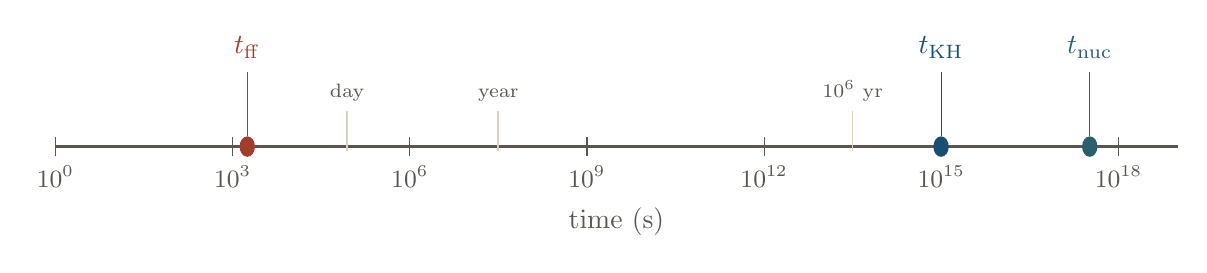
\begin{tikzpicture}[x=0.75cm,y=1cm]
  \draw[muted, line width=0.8pt] (0,0) -- (19,0);
  \foreach \e in {0,3,6,9,12,15,18} { \draw[muted] (\e,0.12) -- (\e,-0.12); \node[below, muted] at (\e,-0.12) {\small $10^{\e}$}; }
  \node[muted] at (9.5,-0.95) {time (s)};
  \foreach \lab/\e in {day/4.937, year/7.499, {$10^6$ yr}/13.499} { \draw[linecol, line width=0.6pt] (\e,-0.05) -- (\e,0.45); \node[above, muted, font=\scriptsize] at (\e,0.45) {\lab}; }
  \foreach \lab/\e/\c in {{$t_{\rm ff}$}/3.248/accent, {$t_{\rm KH}$}/14.996/astroblue, {$t_{\rm nuc}$}/17.514/accent2} { \fill[\c] (\e,0) circle (0.13); \node[\c, above] at (\e,1.0) {\lab}; \draw[\c] (\e,0.13) -- (\e,0.95); }
\end{tikzpicture}
\end{document}
